\section{Resultados}

Los resultados finales que se han obtenido son el enriquecimiento funcional de las poblaciones que fueron generadas aplicando la metodología descrita anteriormente.

En primer lugar, se obtuvo la división de población a través del algoritmo de Louvain, que como se ha observado en la Figura \ref{fig:Grafo_louvain}, existen 5 comunidades bastante pronunciadas.

\begin{figure}[h!]
	\centering
	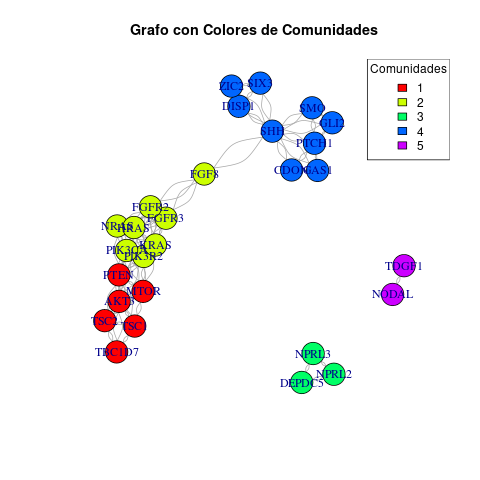
\includegraphics[width=0.8\textwidth]{figures/grafo_colores_comunidades.png}
	\caption{Grafo louvain}
	\label{fig:Grafo_louvain}
\end{figure}

También, se ha obtenido la división por el algoritmo de edge betweenness, que como se ha observado en la Figura \ref{fig:Grafo_between}, son las mismas comunidades pero con una ligera diferencia entre dos comunidades.

\begin{figure}[!]
  \centering
  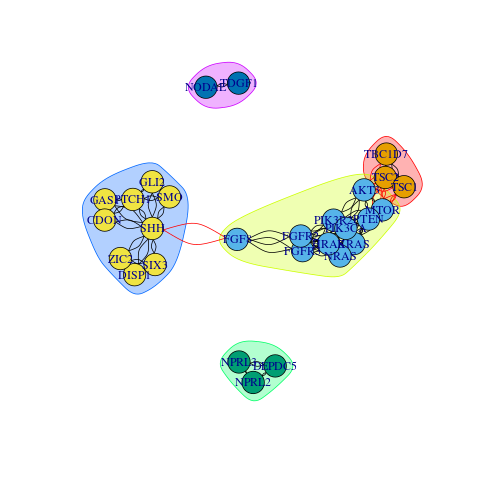
\includegraphics[width=0.8\textwidth]{figures/grafo_alternativo_comunidades.png}
  \caption{Grafo edge betweenness.}
  \label{fig:Grafo_between}
\end{figure}

Para facilitar la comprensión de los diferentes modelos, se muestra en la Tabla \ref{tabla:nodos_enlaces_diferentes} una comparación por nodos. Las filas indican los nodos, la primera columna representa el algoritmo de louvain, y la segunda a la de edge betweenness. Los valores de las celdas indican en que comunidad se encuentra este nodo. Finalmente, en la última columna se muestra si el nodo es asociado a la misma comunidad ("iguales"), o bien si pertenecen a diferentes comunidades ("diferentes").

\newcolumntype{C}{>{\centering\arraybackslash} m{3cm} }
\begin{table}[!]
 	\caption{Descripción de Nodos, Enlaces y Diferentes}
	\centering
	\begin{tabular}{|C|C|C|}
    \toprule
    Nodos & Enlaces & Diferentes \\
    \midrule
     1 & 1 & Iguales \\
     2 & 2 & Iguales \\
     3 & 3 & Iguales \\
    4 & 4 & Iguales \\
     2 & 2 & Iguales \\
     4 & 4 & Iguales \\
    2 & 2 & Iguales \\
     4 & 4 & Iguales \\
     5 & 5 & Iguales \\
     4 & 4 & Iguales \\
     1 & 1 & Iguales \\
     4 & 4 & Iguales \\
     2 & 2 & Iguales \\
     4 & 4 & Iguales \\
     2 & 2 & Iguales \\
     1 & 2 & Diferentes \\
     2 & 2 & Iguales \\
     1 & 2 & Diferentes \\
     2 & 2 & Iguales \\
     1 & 1 & Iguales \\
     3 & 3 & Iguales \\
     1 & 2 & Diferentes \\
     2 & 2 & Iguales \\
     3 & 3 & Iguales \\
    4 & 4 & Iguales \\
     4 & 4 & Iguales \\
     5 & 5 & Iguales \\
     4 & 4 & Iguales \\
 		\bottomrule
   \label{tabla:nodos_enlaces_diferentes}
 	\end{tabular}
\end{table}

Posteriormente, se calculó la modularidad y se representó en la Figura \ref{fig:comparacion_grafos}.

\begin{figure}
  \centering
  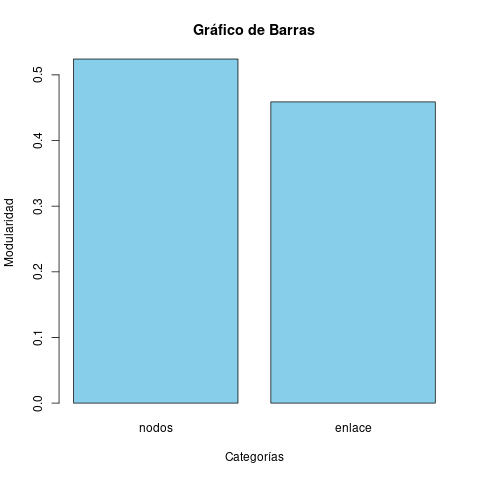
\includegraphics[width=0.8\textwidth]{figures/comparacion_grafos.png}
  \caption{Comparación con modularidad.}
  \label{fig:comparacion_grafos}
\end{figure}

Finalmente, se obtuvo el enriquecimiento funcional del mejor algoritmo basándonos en la modularidad. Para representar las funciones asociadas a cada comunidad, se han creado tantas tablas como comunidades (ver Tablas \ref{tabla:genes_funciones_1}, \ref{tabla:genes_funciones2},  \ref{tabla:genes_funciones3}, \ref{tabla:genes_funciones4} y \ref{tabla:genes_funciones5}), en las que, en la primera columna, se muestra el conjunto de nodos dentro de la comunidad con una función en común, y en la segunda columna, la propia función.

\begin{table}[!]
 	\caption{Descripción de Genes y Funciones de la comunidad 1}
	\centering
	\begin{tabular}{|C|C|}
    \toprule
    \textbf{Genes} & \textbf{Funciones} \\
    \midrule
    TSC2, TSC1, MTOR, PTEN, TBC1D7, AKT3 & negative regulation of intracellular signal transduction (GO:1902532) \\
    \bottomrule
    \label{tabla:genes_funciones_1}
 	\end{tabular}
\end{table}

\begin{table}[!]
 	\caption{Descripción de Genes y Funciones de la comunidad 2}
	\centering
	\begin{tabular}{|C|C|}
    \toprule
    \textbf{Genes} & \textbf{Funciones} \\
    \midrule
    PIK3R2, KRAS, PIK3CA, FGF8, FGFR3, NRAS, HRAS, FGFR2 & MAPK cascade (GO:0000165) \\
    PIK3R2, KRAS, PIK3CA, FGF8, FGFR3, NRAS, HRAS, FGFR2 & Transmembrane receptor protein tyrosine kinase signaling pathway (GO:0007169) \\
    PIK3R2, KRAS, PIK3CA, FGF8, FGFR3, NRAS, HRAS, FGFR2 & Positive regulation of intracellular signal transduction (GO:1902533) \\
    \bottomrule
    \label{tabla:genes_funciones2}
 	\end{tabular}
\end{table}



\begin{table}[!]
 	\caption{Descripción de Genes y Funciones de la comunidad 3}
	\centering
	\begin{tabular}{|C|C|}
    \toprule
    \textbf{Genes} & \textbf{Funciones} \\
    \midrule
    NPRL2, NPRL3, DEPDC5 & Cellular response to amino acid starvation (GO:0034198) \\
    NPRL2, NPRL3, DEPDC5 & Negative regulation of TOR signaling (GO:0032007) \\
    NPRL2, NPRL3, DEPDC5 & Regulation of TOR signaling (GO:0032006) \\
    NPRL2, NPRL3, DEPDC5 & Cellular response to starvation (GO:0009267) \\
    NPRL2, NPRL3, DEPDC5 & Negative regulation of intracellular signal transduction (GO:1902532) \\
    \bottomrule
    \label{tabla:genes_funciones3}
 	\end{tabular}
\end{table}

\begin{table}[!]
 	\caption{Descripción de Genes y Funciones de la comunidad 4}
	\centering
	\begin{tabular}{|C|C|}
    \toprule
    \textbf{Genes} & \textbf{Funciones} \\
    \midrule
    SMO, SIX3, DISP1, SHH, GAS1, PTCH1, GLI2, ZIC2, CDON & Smoothened signaling pathway (GO:0007224) \\
    SMO, SIX3, DISP1, SHH, GAS1, PTCH1, GLI2, ZIC2, CDON & Negative regulation of transcription, DNA-templated (GO:0045892) \\
    \bottomrule
    \label{tabla:genes_funciones4}
 	\end{tabular}
\end{table}



\begin{table}[!]
 	\caption{Descripción de Genes y Funciones de la comunidad 5}
	\centering
	\begin{tabular}{|C|C|}
    \toprule
    \textbf{Genes} & \textbf{Funciones} \\
    \midrule
    NODAL, TDGF1 & BMP signaling pathway (GO:0030509) \\
    NODAL, TDGF1 & Cellular response to BMP stimulus (GO:0071773) \\
    NODAL, TDGF1 & Transmembrane receptor protein serine/threonine kinase signaling pathway (GO:0007178) \\
    NODAL, TDGF1 & Positive regulation of protein phosphorylation (GO:0001934) \\
    NODAL, TDGF1 & Positive regulation of cell proliferation (GO:0008284) \\
    NODAL, TDGF1 & Regulation of apoptotic process (GO:0042981) \\
    NODAL, TDGF1 & Regulation of transcription from RNA polymerase II promoter (GO:0006357) \\
    \bottomrule
    \label{tabla:genes_funciones5}
 	\end{tabular}
\end{table}




